\cleardoublepage

\chapter{Background}
\label{Ch2:Back}

\section{Metamorphic testing in classical computing}
\label{Ch2.1:Metamorphic}

\section{Quantum computing}
\label{Ch2.2:Quantum}
Elements to be included:
\begin{itemize}
    \item Relaxation time
\end{itemize}

\newpage

\section{Testing in Quantum}
\label{Ch2.3:TQuantum}

After providing a brief introduction to quantum computing, let us allocate some time to delve into the latest developments in the field of quantum testing. This section will be divided into two different perspectives. Firstly, we will explore the testing of Quantum Platforms, with a specific focus on Qiskit and how it can evolve for different platforms. Subsequently, we will continue with various approaches and techniques for testing quantum programs, hereafter referred to as QP.

\subsection{Quantum computing platforms}
\label{Ch2.3.1:TPlat}

As mentioned earlier, we will begin by examining the testing of quantum platforms. We will introduce these approaches in chronological order and the authors will even assess how they compare to each other, observing improvements over time.

\subsubsection{QDiff}
\label{Ch2.3.1:QDiff}

QDiff, differential testing of quantum software stacks (QSS), is the approached presented by Jiyuan Wang et all. in their 2021 article titled \textit{"QDiff: differential testing of quantum software stacks"}\cite{wang2021qdiff}, they introduce it as a novel differential testing technique for QSS.\newline

Their motivation behind this work arises from the increasing interest in quantum computing and the development of QSS as a high-level languages for quantum programming. These languages aim to shield users from the mathematical and physical complexities inherent in quantum computing. Another motivation is to offer a potential solution for identifying failures within QSS, which aids in resolving the confusion and incoherence that often arises when a user reports bugs. When reviewing the collection of issues reported for each QSS, these problems frequently reveal inconsistencies in identifying the potential source of the bug or determining whether the issue originates from the probabilistic or noisy nature of quantum indeterminacy. \newline

The authors idea is to be able to perform testing in the three most widely used QSS \cite{larose2019overview} at that time: Qiskit, Cirq and Pyquil. Now, let us explore the workflow and key innovations in  QDiff, which will include their propose solutions for technical challenges that complicate testing within QSS.

\newpage
\begin{itemize}
    \item QP generator: In order to fulfil our needs while testing QSS, we need to generate semantically equivalent programs. The authors proposed a set of equivalent gate transformation rules designed to preserve program semantics. These seven rules have been derived from a detail analysis of each gate and their behaviour when deployed sequentially.
    \begin{figure}[H]
        \centering
        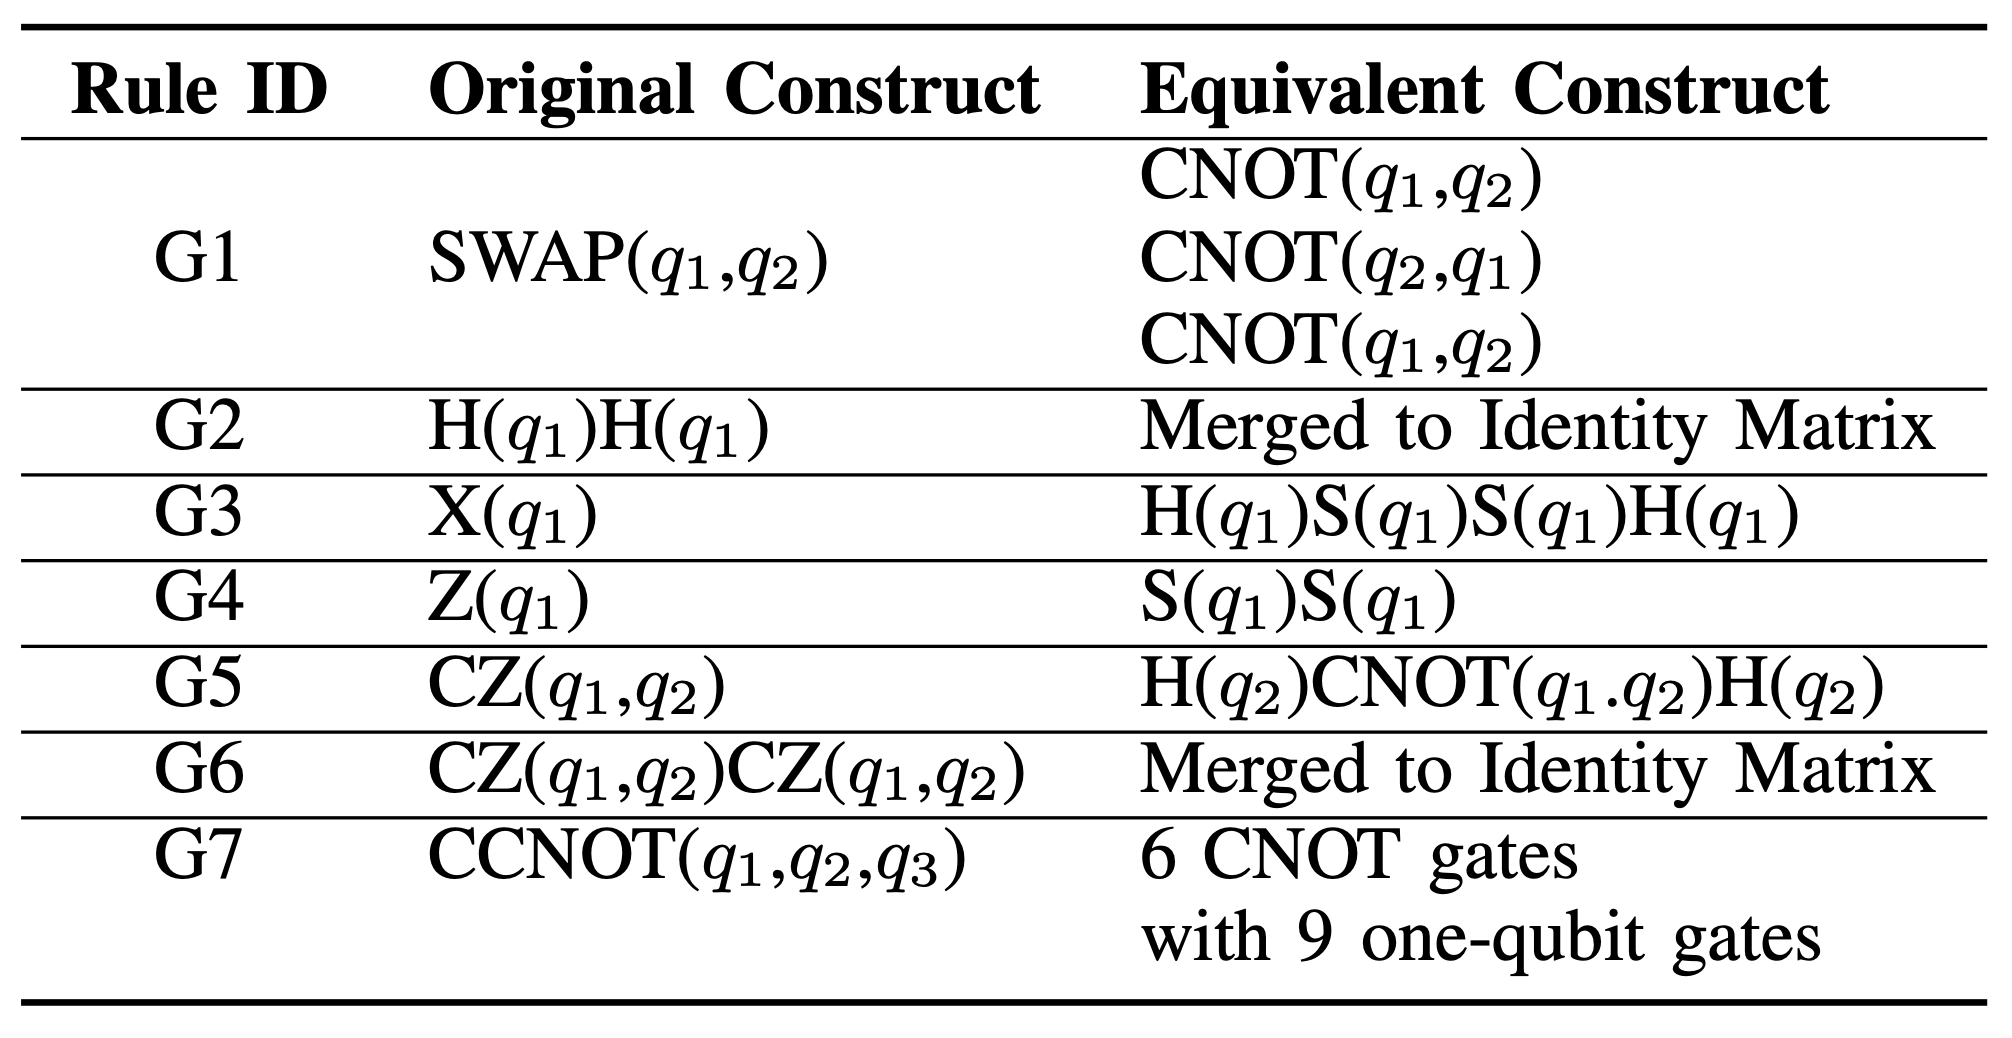
\includegraphics[width=0.6\textwidth]{TFM/photos/QDiffRules.png}
        \caption{Semantic preserving rules \cite{wang2021qdiff}} 
        \label{Fig:QDiffRules}
    \end{figure}

    It does follow by mutation modifications: NEEDS CHECKING, as first it says  we apply preserving then mutations and after the opposite.

    \item Filtering process of circuits depending on the worth of running. Discussing T1 time, number of gates...

    \item Comparing results from two equivalent quantum programs. Check for the reasoning of number of executions needed and how they may use K-S test.
    
\end{itemize}

\newpage
\subsubsection{MorhpQ}
\label{Ch2.3.1:MorphQ}
Matteo Paltenghi and Michael Pradel presented in May 2023 their latest work on testing QQS, introducing metamorphic testing as a novel approach for quantum platforms. Their innovative method involves the design of metamorphic rules for Qiskit.3 Their article, titled: \textit{"MorphQ: Metamorphic testing of the qiskit quantum computing platform"} \cite{paltenghi2023morphq}, further develops this concept, presenting a fresh perspective on generating quantum programs using a defined grammar. This advancement brings us closer to the idea of automating the testing process, eliminating the need for a library of quantum programs as generation seed, which was the traditional approach up to this point.\newline

MorphQ will focus on Qiskit, as quantum platform, employing metamorphic testing to address specific challenges presented in quantum computing. The oracle problem will be avoided as it will be resolved by the use of MR, eliminating the need for a detailed specification of expected input behaviour. Let us provide a general overview of MorphQ as presented by the authors, then we will focus on the key innovations within each of its distinct components .

\begin{figure}[H]
        \centering
        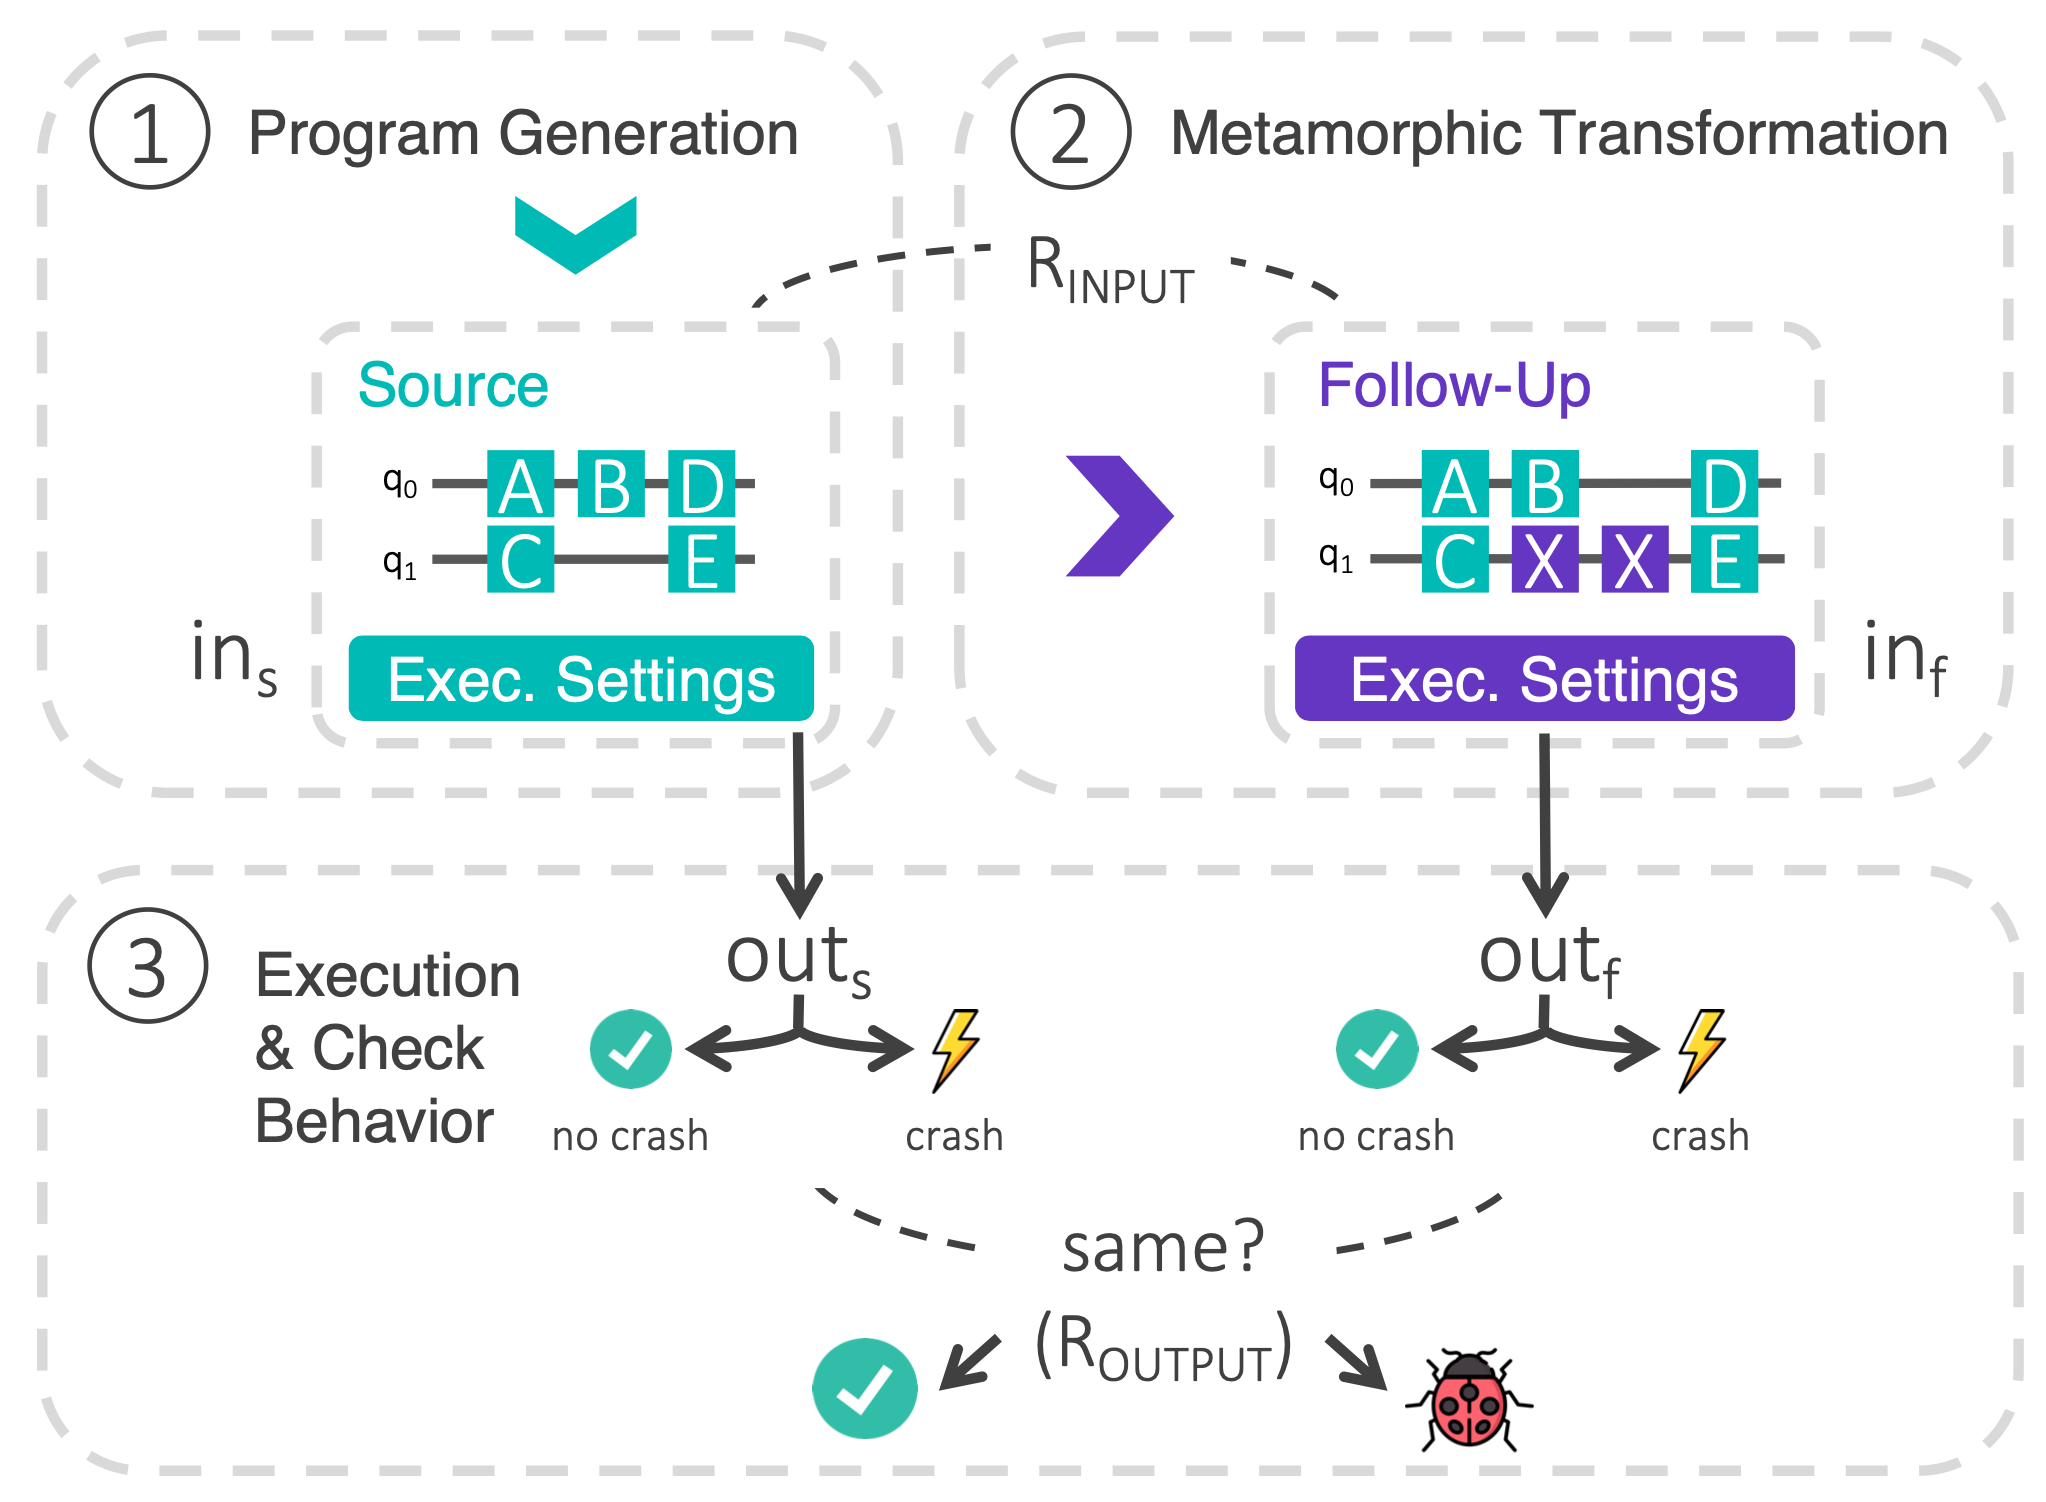
\includegraphics[width=0.6\textwidth]{TFM/photos/MorphQOverview.png}
        \caption{MorphQ overview \cite{paltenghi2023morphq}} 
        \label{Fig:MorphQOverview}
\end{figure}

As previously mentioned, one of the authors' significant contributions lies in their approach to program generation. Since the focus is on testing the quantum platform, the primary objective of this proposal is to create syntactically correct quantum programs, thus preventing execution crashes. These this automating generated programs will serve as test suit for the QSS. To begin, Paltenghi and Pradel introduced the grammar that will guide the program generation process. This grammar follows the typical recursive structure found in computing. A subset of it is illustrated in Figure \ref{Fig:MorphQGrammar}, as provided by the authors in their paper. You can access all the related information about the grammar and the rest of the article on their \hyperlink{https://github.com/sola-st/MorphQ-Quantum-Qiskit-Testing-ICSE-23}{GitHub} page. (Visible link, hided link, footnote, both?)

\begin{figure}[H]
        \centering
        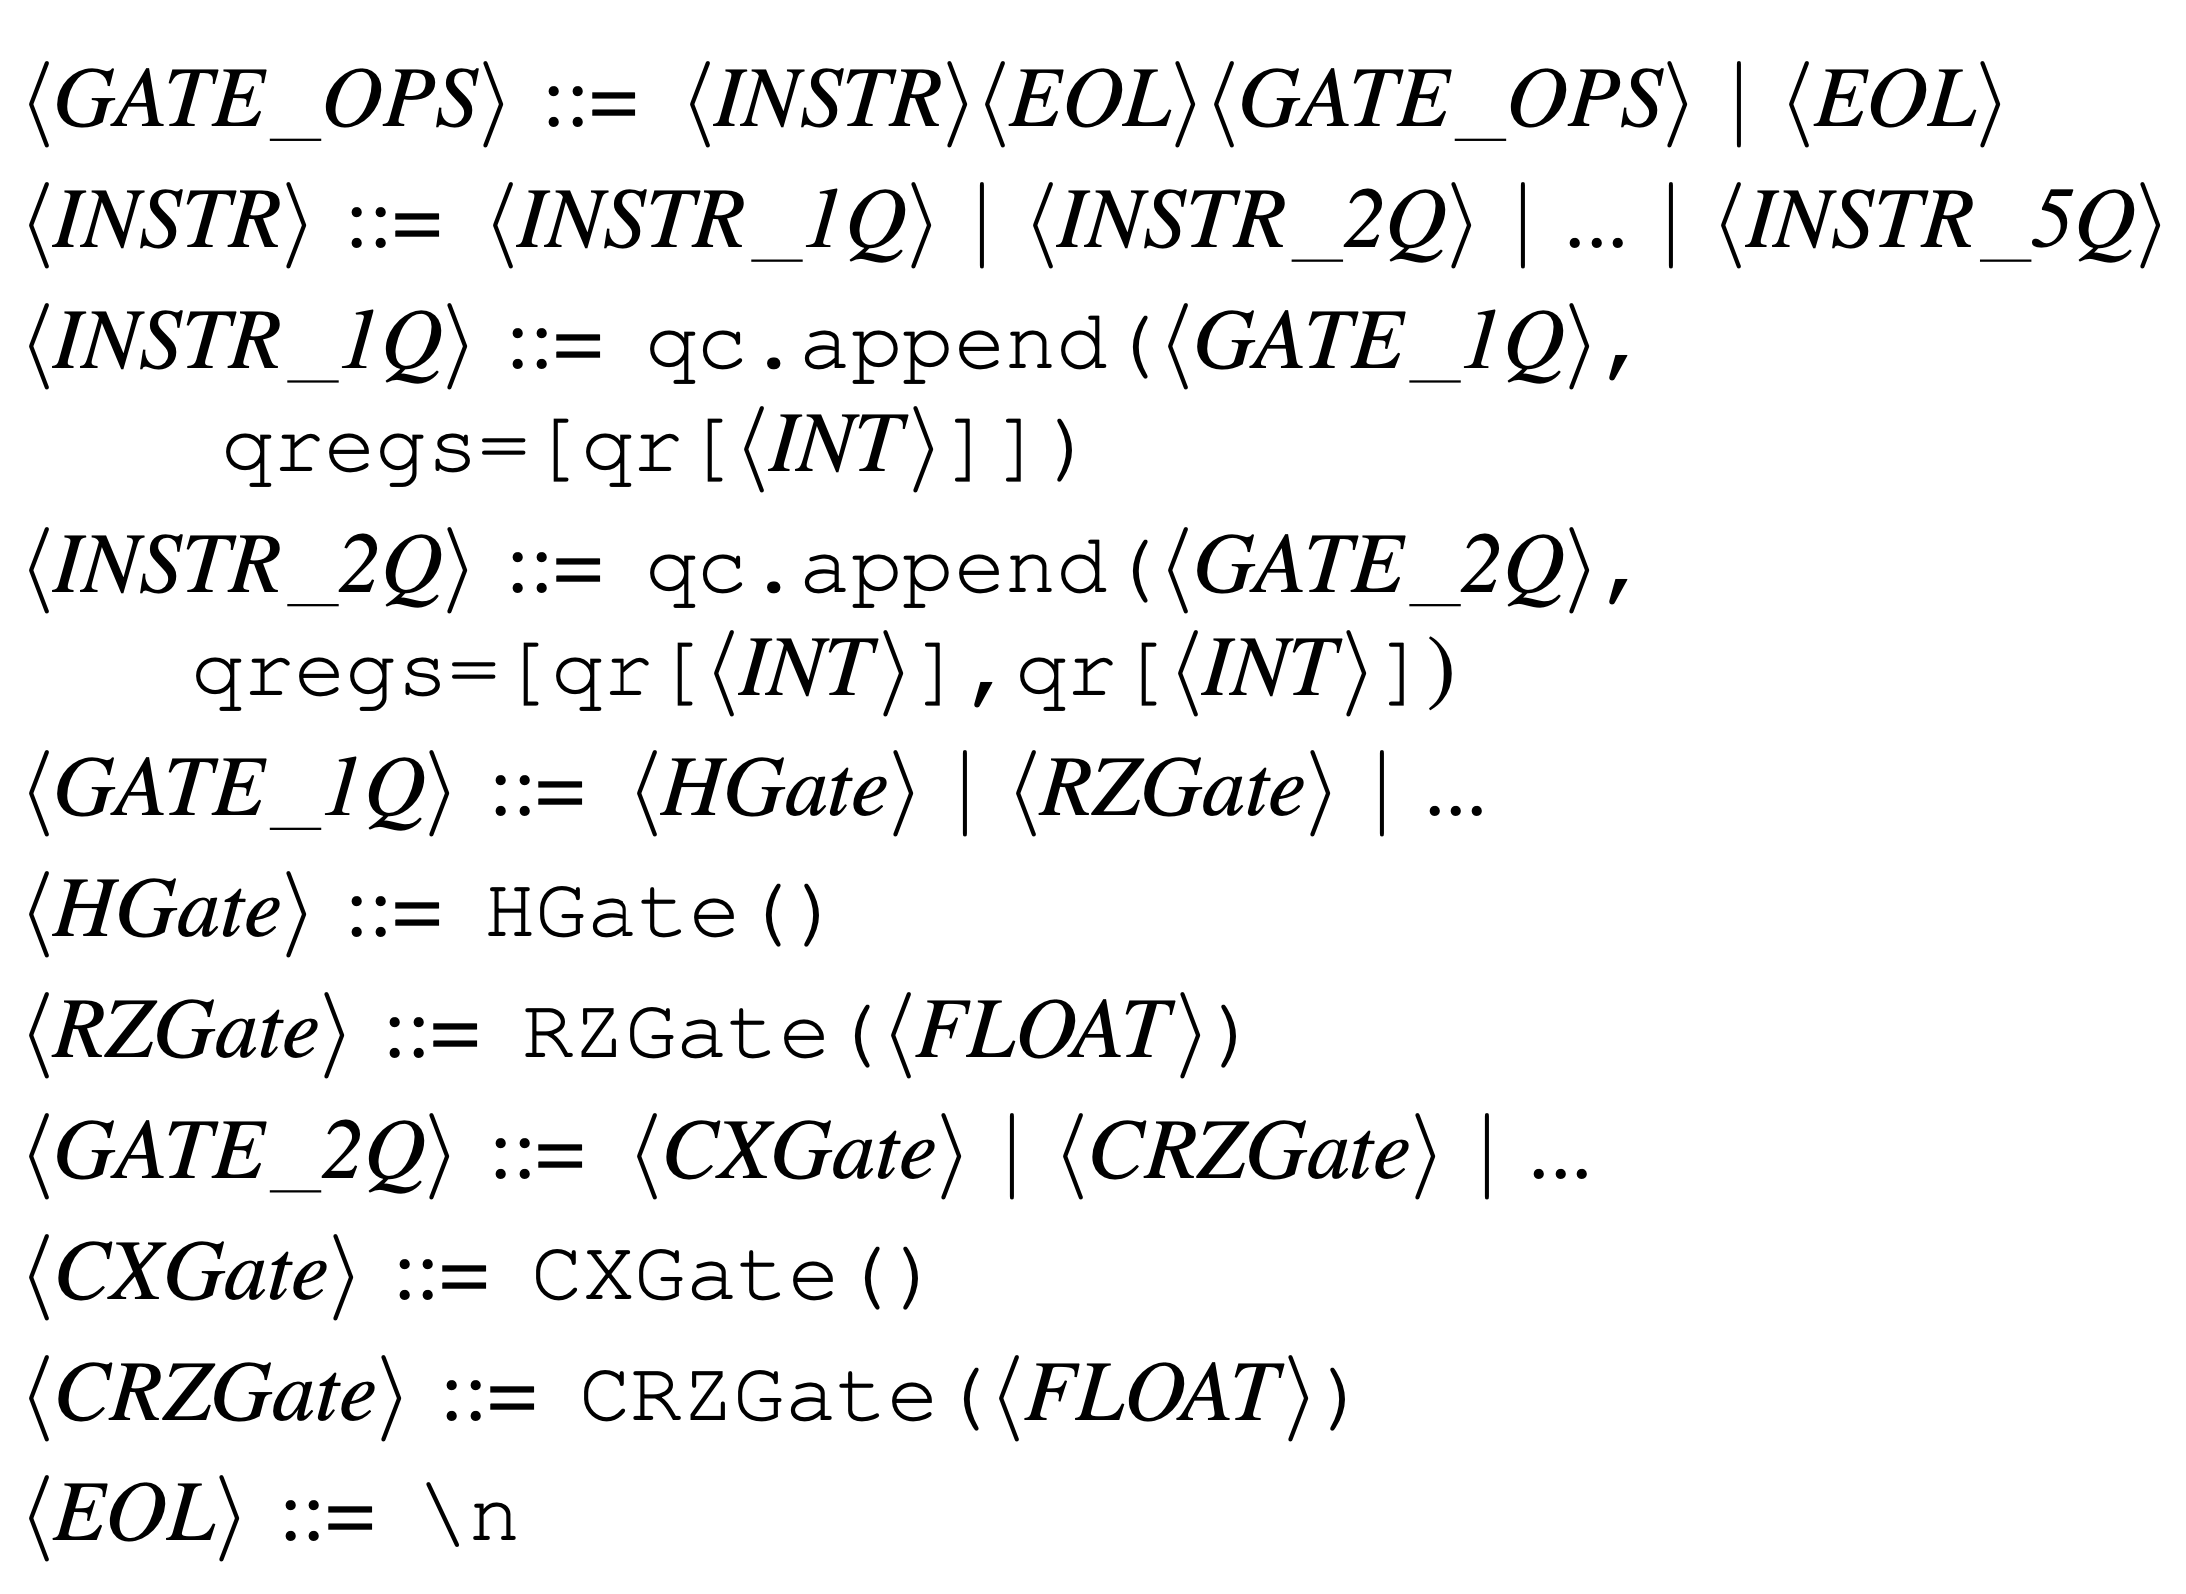
\includegraphics[width=0.6\textwidth]{TFM/photos/MorphQGrammar.png}
        \caption{Subset of the QP generation grammar \cite{paltenghi2023morphq}} 
        \label{Fig:MorphQGrammar}
\end{figure}

The purpose of defining this grammar is to ensure that invalid quantum programs are avoided. A random approach would not be ideal, as it would likely generate a high number of invalid programs. Additionally, the authors will impose a constraint on the number of gates per program, limiting it to 30. Higher amount of gates can increase considerably the execution time due to the complexity of quantum operations. Their commitment towards keeping execution times within reasonable limits, lies in the decision of the authors to only use simulators, where the size of the matrix defining a single operator grows exponentially with the number of qubits involved.\newline

Once we have been able to generate the source input for the testing desired, the authors defined the metamorphic rules that Qiskit should fulfil classifying them in 3 categories: Circuit transformation which modify the circuit, representation transformations which change the intermediate representation of QP and execution transformations, which affect the execution environment, we could observe this metamorphic rules in Figure \ref{Fig:MorphQMR}. 

\begin{figure}[H]
        \centering
        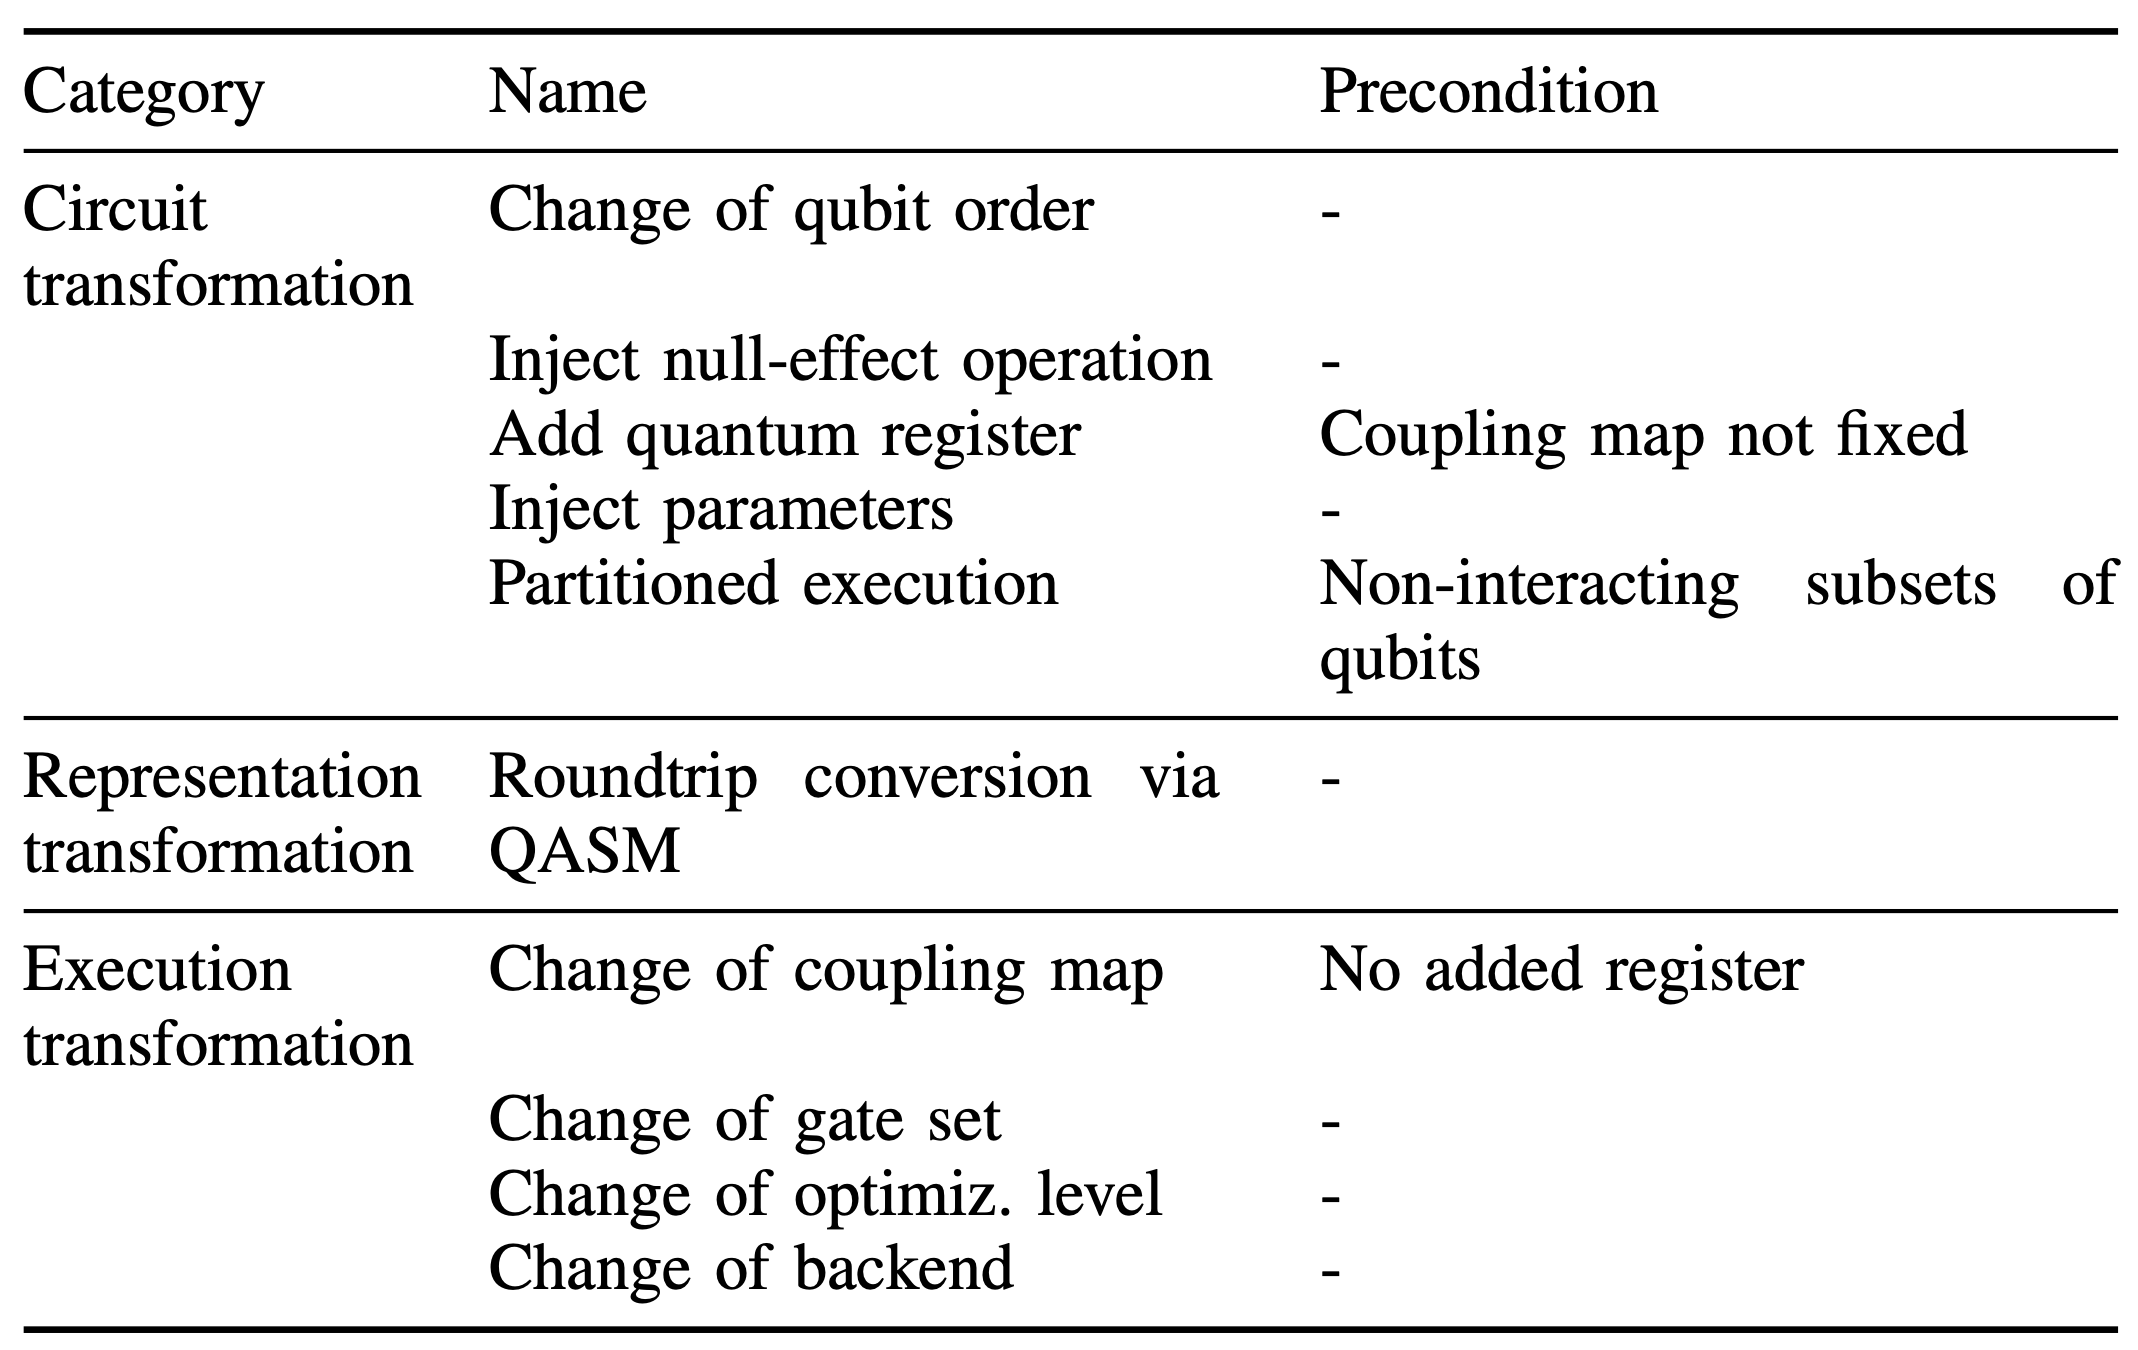
\includegraphics[width=0.6\textwidth]{TFM/photos/MorphQMR.png}
        \caption{Qiskit MR used by QMorph \cite{paltenghi2023morphq}} 
        \label{Fig:MorphQMR}
\end{figure}

The expected relationship between source and follow-up outputs is "equivalence", with the only exception of non-semantic-preserving transformations, specifically, the change of qubit order and partitioned execution which will need a posterior treatment before comparing behaviours. This is why we will continue applying metamorphic transformations unless one of the exceptions mentioned above is introduced. This transformations are executed through python AST or/and sectioning source code with python matching technique, adding needed elements and reconstructing the code.\newline

In the final step of MorphQ, which involves execution and behaviour checks, the primary assessment is crash check. Identifying a crash in the follow-up program marks a critical failure. As we are all aware, when executing quantum programs without accounting for quantum noises, the result can be non-deterministic linked to the final state amplitudes, reflecting the well-known probabilistic nature of quantum measurement. Consequently, we would need to execute the programs a specific number of shots to compare two different distributions and decide if the output is "equivalent" or we have possibly found a failure. To determine this 
required number of executions, the authors follow the same technique as the one used in QDiff, employing the \textbf{L1 norm }\cite{chan2014optimal}. The distribution are compared using Kolmogorov-Smirnov test (p-value < 5\%)\newline
 
Another noteworthy aspect is the management of warning messages related to crashes. The authors implemented a semi-automatic clustering approach for these warnings, aiming to abstract from program-specific references. Afterwards, a random selection process is applied to each cluster, and the chosen programs undergo manual inspection. During these inspections, transformations are reversed step by step until the one responsible for the fault is reached. Then, they use \textbf{delta debugging} until they identify the minimal sequence of operations to trigger the crash. \newline

Let us summarise the key results and contributions of MorphQ, keeping in mind that the experiments were constrained by a 48-hour execution time-frame. The authors also adapted QDiff to the same execution time-frame to be able to compare results.

\begin{itemize}
    \item QP generator:
    \begin{itemize}
        \item Automatically generated 8360 quantum programs .
        \item Source-QP executed without crashing.
        \item Wide range of programs produced (Figure \ref{Fig:MorpgQDiverQP}). 
        \item Higher code coverage vs QDiff: 8.1\% vs 6.1\% 
    \end{itemize}
    \item 13 bugs discovered in the latest version of Qiskit.
    \item Follow-up QP behaviour analysis:
    \begin{itemize}
        \item Crashed in 23.2\% of the cases,with only 56 programs showing a distribution difference.
        \item Demonstrated wider diversity compared to QDiff, as measured by unique API calls.
        \item \textit{Roundtrip conversion via QASM} and \textit{Inject null-effect operations} are the most effective MR, althogh a combination of several MR will produce better results, exposing 8 out of 13 bugs (Figure \ref{Fig:MorpgQDiverQP}). 
        \item Non-crashing follow-up QP: Upon evaluating the 56 programs, it was determined that the differences in distribution were due to randomness, which is plausible given the test's significance level.
    \end{itemize}
    \item False positive: MorphQ may generate false positive warnings because the MR do not always hold in practice, even when is theoretically sound. This can occur when applying the \textit{Change of gate set}. In Qiskit, A* algorithm is used to find equivalent gates, although exploring all possibilities is impractical. Therefore, we might encounter the warning \textit{"Unable to map source basis to target basis"}, which  could be recognised as a limitation of the platform.
\end{itemize}

\begin{figure}[!tbp]
  \centering
  \begin{minipage}[b]{0.36\textwidth}
    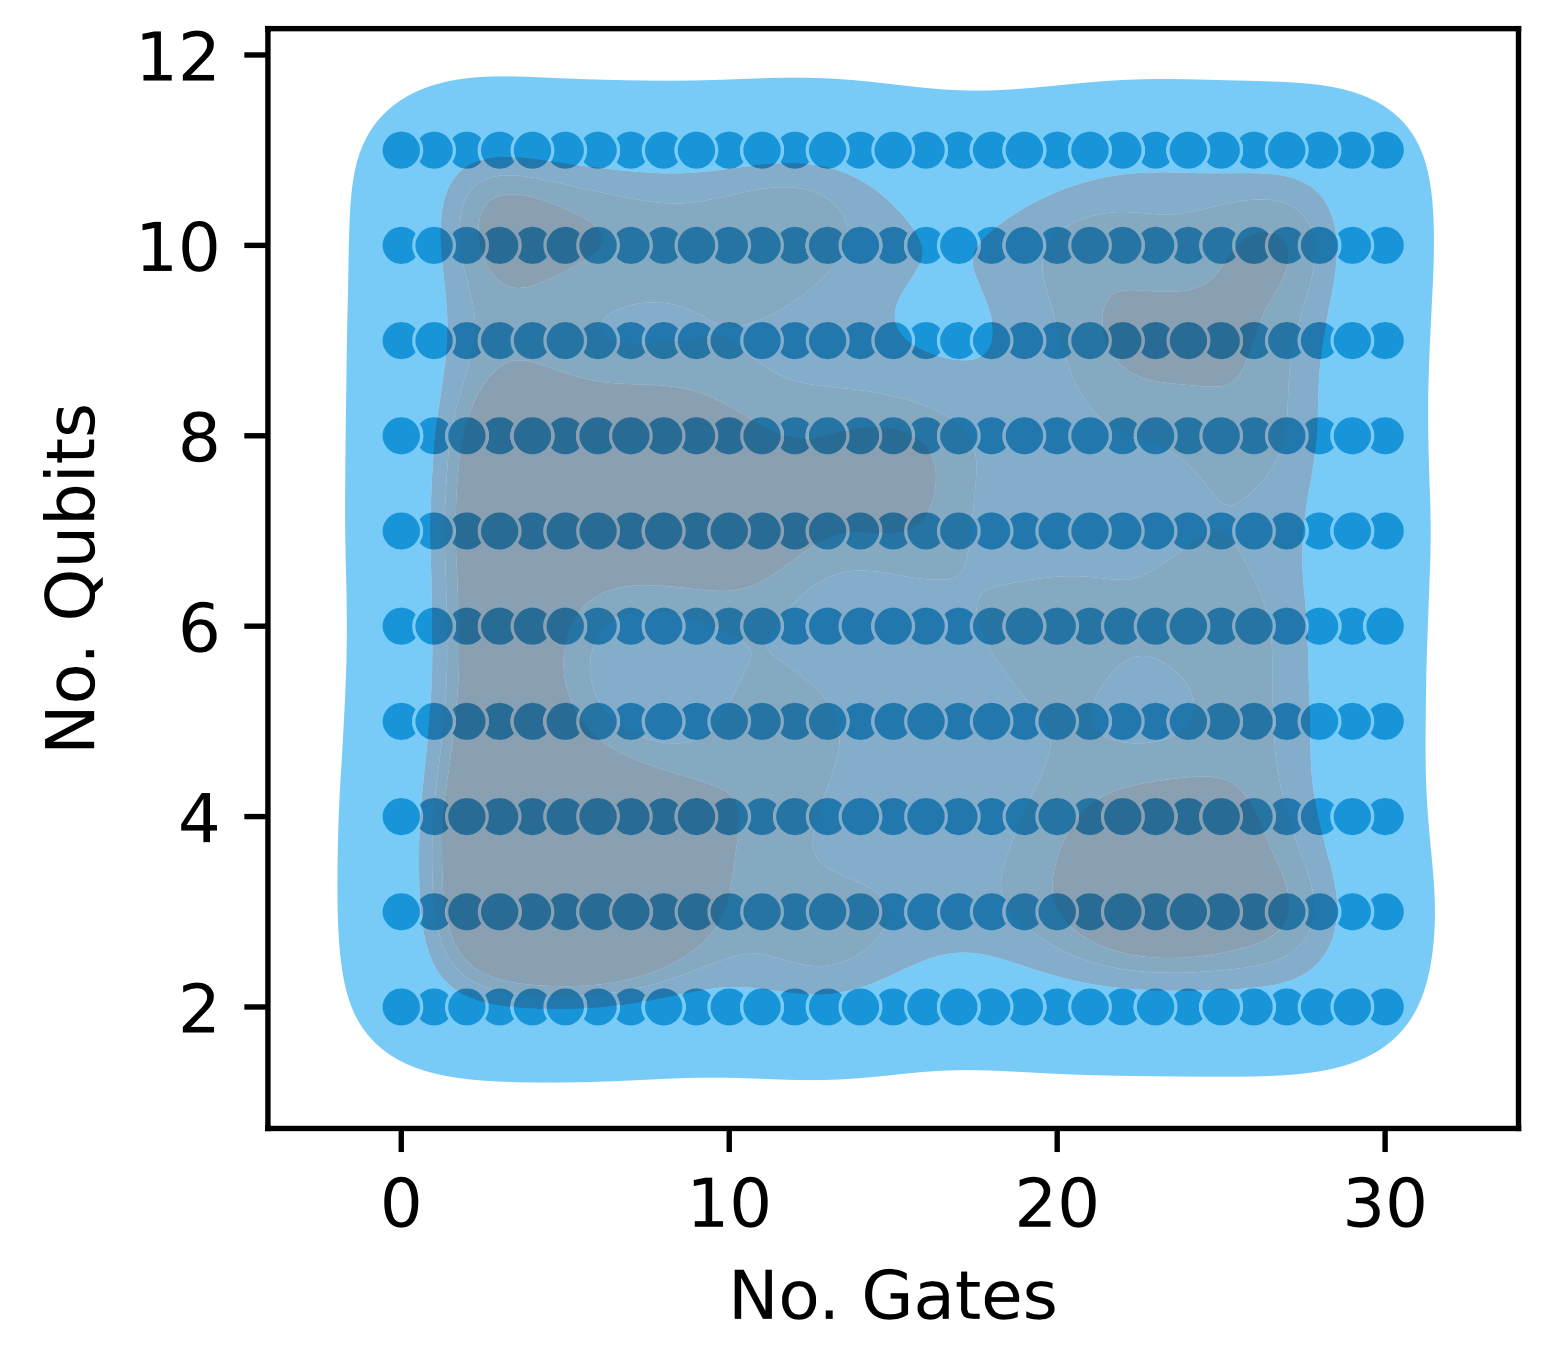
\includegraphics[width=\textwidth]{TFM/photos/MorpgQDiverQP.png}
    \caption{QP diversity \cite{paltenghi2023morphq}.} 
    \label{Fig:MorpgQDiverQP}
  \end{minipage}
  \hfill
  \begin{minipage}[b]{0.55\textwidth}
    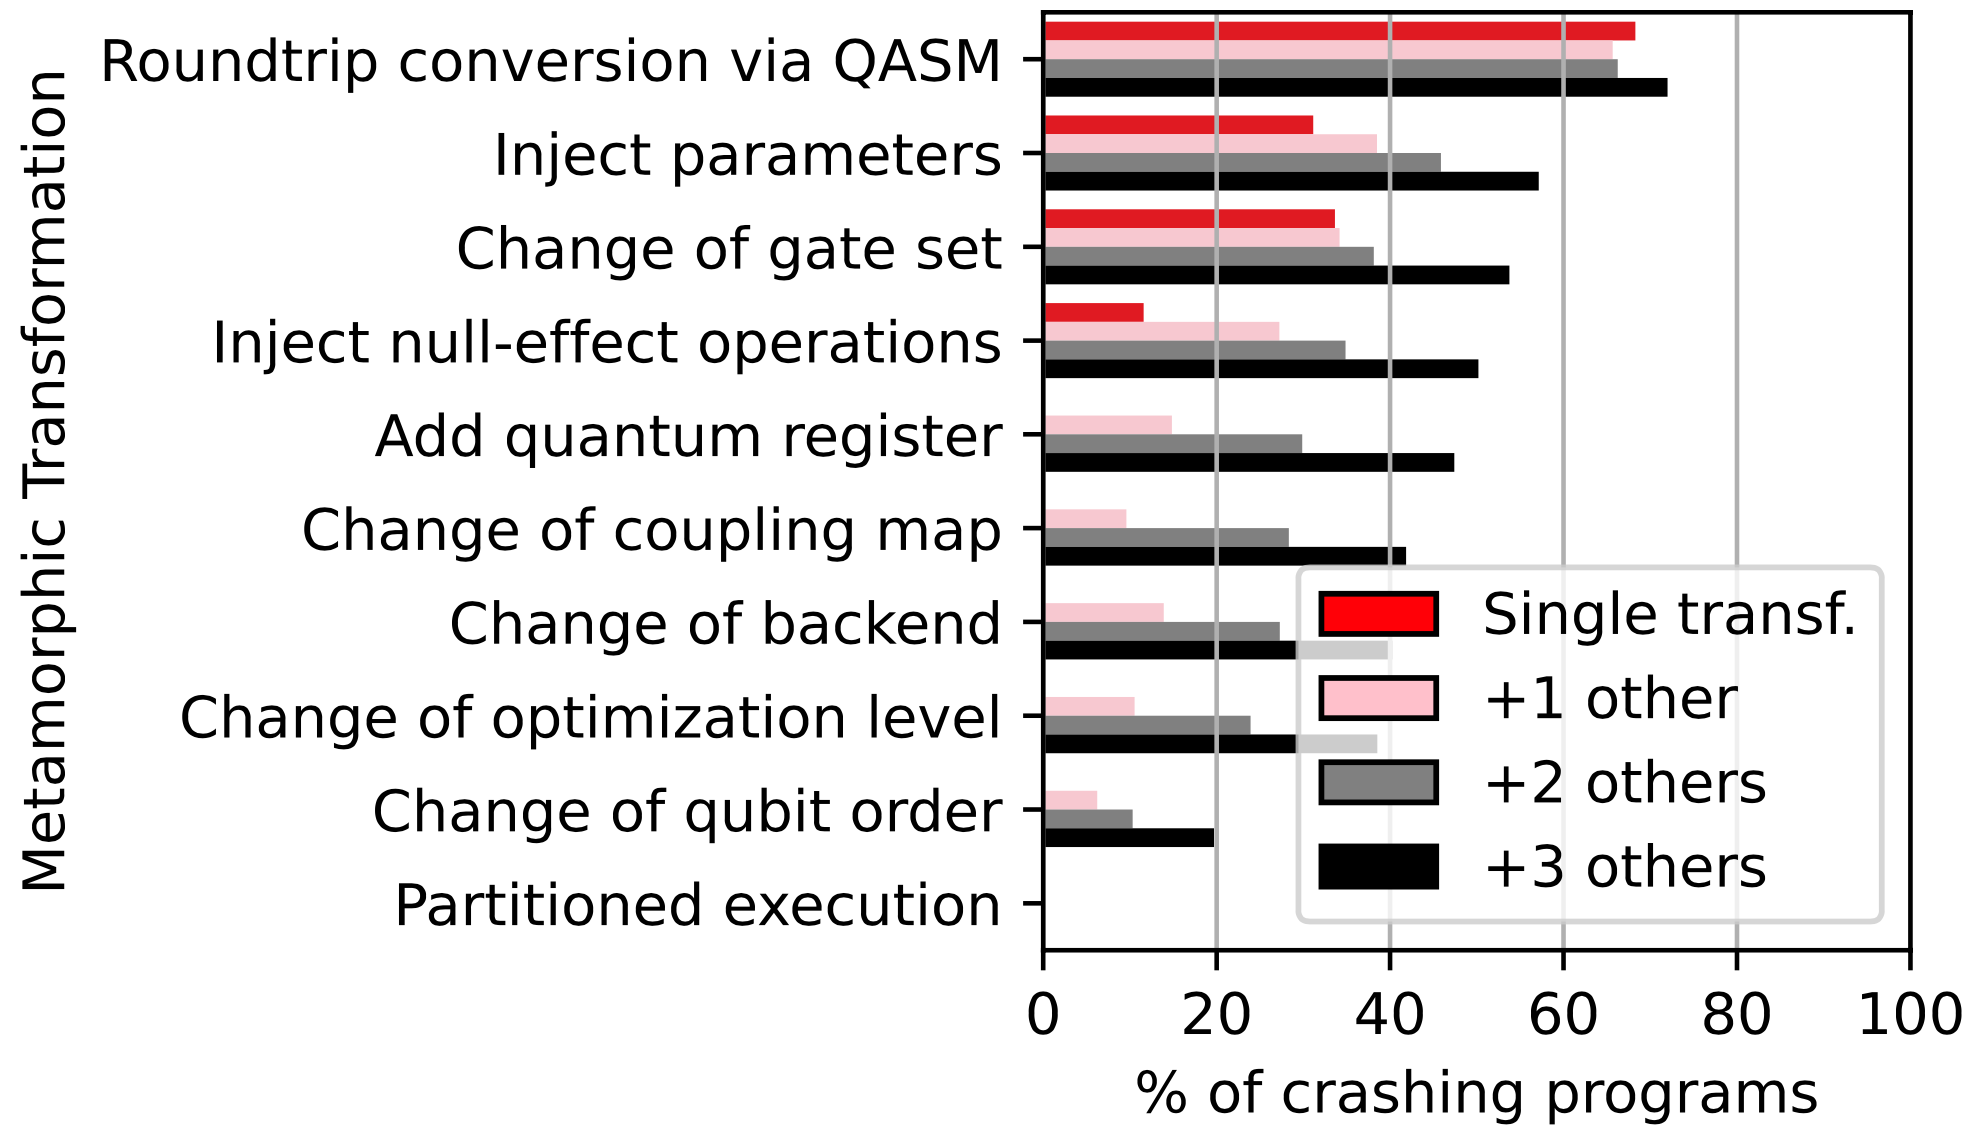
\includegraphics[width=\textwidth]{TFM/photos/MorphQMRCrash.png}
    \caption{MR analysis in follow-up QP \cite{paltenghi2023morphq}.} 
    \label{Fig:MorphQMRCrash}
  \end{minipage}
\end{figure}

\subsection{Quantum computing programs}
\label{Ch2.3.2:TQP}
After considering some of the latest results regarding testing of quantum platforms and the diverse challenges they have encountered and overcame, we will shift our focus towards testing our QP implementations. This presents a different challenge where we have an algorithm or specification and an implementation that should represent that algorithm. We will explore the recent developments and analyse different techniques used for testing an implementation (QP) of a given algorithm.

\vspace{10pt}

\subsubsection{QMutPy}
\label{Ch2.3.2:QMutPy}
The initial approach we are presenting was authored by Fortunato, D. et all in 2022 in their article titled "\textit{Mutation testing of quantum programs: A case study with qiskit}"\cite{fortunato2022mutation}. In this work, they explore mutation testing on QP with the extension of the MutPy library by introducing new quantum mutation operators. This article can be divided into two distinct sections. The first section focuses on the introduction of QMutPy and the initial experiments. The second section delves deeper into the previous results to identify potential causes and solutions. The authors implement some of these solutions to determine if they are on the right path. \newline

First, let us understand what QP are going to be tested and why did the authors choose this library. The oracle problem was one of the challenges discussed earlier, where given an input, we need the expected behaviour. In this article, the authors have decided to prioritise and initially focus on this new approach for QP testing. To accomplish this, they opted to use Qiskit-Aqua's repository, which has since been moved to Qiskit-Terra \footnote{\url{https://github.com/Qiskit/qiskit-aqua/\#migration-guide}}.This repository provides the implementation of 24 QP along with their respective test suites. In these repository, you can discover a variety of programs, including pure classical, hybrid, and pure quantum programs.\newline

Similarly, they carefully selected the tool they believed would be the most suitable for implementing their ideas about quantum mutation testing. Their criteria included support for Python programs, testing frameworks, mutation operators, and the capability to generate appropriate reports. For that reason, they choose MutPy, as it fulfils their specific needs. Now, let us see how they develop these new quantum mutation operators, expanding the library mentioned earlier and naming it QMutPy.\newline

They have introduced in QMutPy 5 quantum mutation operators, QMO:
\begin{itemize}
    \item Quantum gate replacement, QRG.
    \item Quantum gate deletion, QRD.
    \item Quantum gate insertion, QRI.
    \item Quantum measurement insertion, QMI.
    \item Quantum measurement deletion, QMD.
\end{itemize}

\vspace{5pt}
These new operators are designed to capture the main errors that can occur during the implementation of an algorithm. The key concept around QMO is gate equivalence. We will consider two gates to be syntactically equivalent if and only if the number and type of the arguments are identical. The authors have identified 40 gates with at least one syntactical equivalent gate. As an example, gate h would have the following equivalent gates: x, y, z, i, id, s, sdg, sx, t and tdg. In their article \cite{fortunato2022mutation}, the authors illustrated all equivalence gates in Figure 1.  \newline

There is no need to provide an explanation for the mutant operators, as they are inherently self-explanatory.  However, let us dig into a more comprehensive understanding of gate operators. As mentioned earlier, the fundamental concept that makes these operators effective is gate equivalence. Whenever we encounter a gate addition (denoted by ".append()"), and we intend to employ QRG or QRI, we will either replace the existing gate with a syntactically equivalent one or simply add a new gate that preserves the syntax of our program. The process will generate as many mutants as there are syntactically equivalent gates. All of these modifications are implemented using Python's Abstract Syntax Tree (AST).\newline

QMutPy workflow, analogous to MutPy:
\begin{itemize}
    \item Loads QP source code and test suite.
    \item Executes test suite on the unmutated QP.
    \item Applies mutant operators, including QMO.
    \item Executes test suite on all mutated QP and provides a summary of results.
\end{itemize}

Because the works in quantum mutation \cite{wang2021qdiff}\cite{mendiluze2021muskit}\cite{ali2021assessing} were in a preliminary state, the authors opted to compare MutPy and QMutPy by running experiments on the same set of quantum programs and test suites. The experiment's metrics will be assessed through two distinct approximations of the mutation score. The first one follows the classical interpretation\cite{jia2010analysis}, while the second allows for the potential achievement of 100\% mutantion score. This will be achieved by excluding from the total mutants generated those that haven't been executed.\newline

NEED understanding on last step of MutPy/QMutPy

\subsubsection{Quito}
\label{Ch2.3.2:Quito}

\subsubsection{QSharpCheck}
\label{Ch2.3.2:QSharpCheck}

\section{Future work}
\label{Ch2.4:FutureWork}
